% !TeX root = ../presentation.tex

{
    \metroset{sectionpage=none}
    \section{Einleitung}
}

\begin{frame}{Einleitung}
    \begin{columns}
        \begin{column}{0.7\textwidth}
            \begin{itemize}
                \item Daten sind überall, sofort verfügbar und weiterleitbar
                \item für alle Geschäftsprozesse notwendig,\\
                    \enquote{Nebenprodukt} $\to$ strategische Ressource~\cite{mollerIndustrialDataEcosystems2024}
                
                \item<2-> \alert{Data Sharing}: anderen Zugriff auf Daten gewähren, auf die sie selbst keinen hätten~\cite{mollerIndustrialDataEcosystems2024}
                
                \item<3-> viele Bedenken beim Teilen von Daten~\cite{mollerIndustrialDataEcosystems2024}
                \begin{itemize}
                    % Angst vor unberechtigter Weitergabe
                    % Missbrauch von Daten
                    % Kontrollverlust
                    
                    \item<4->[$\Rightarrow$] zurückhaltendes Data Sharing
                \end{itemize}

            \end{itemize}
        \end{column}

        \begin{column}{0.3\textwidth}<2->
            \begin{figure}
                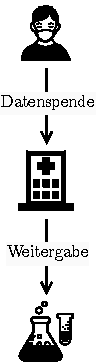
\includegraphics[height=6cm]{./assets/example_vertical.drawio.pdf}
                % TODO: ETL ausschreiben
                % aufwendig
                \caption{Beispiel}
            \end{figure}
        \end{column}
    \end{columns}
\end{frame}


\begin{frame}{Einleitung II}
    \vspace{1em}

    \begin{figure}
        \centering
        \begin{subfigure}{0.5\textwidth}
            \centering
            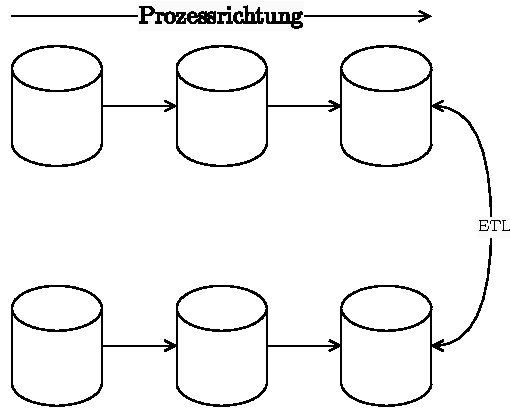
\includegraphics[height=5cm]{./assets/process_view.drawio.pdf}
        \end{subfigure}
        % aktuell findet Entw. wie folgt statt
        % - für einen bestimmten Prozess brauche ich folgende Daten
        % - dafür spezielle Datenspeicher entwerfen und entlang einer Prozesskette integrieren
        % - zwei Endresultate integrieren, bspw. Krankschreibung von Krankenkasse und Arbeitgeber
        %
        % wo wir hin wollen, sind Daten-getriebene Prozesse
        \only<2->{
            \begin{subfigure}{0.4\textwidth}
                \centering
                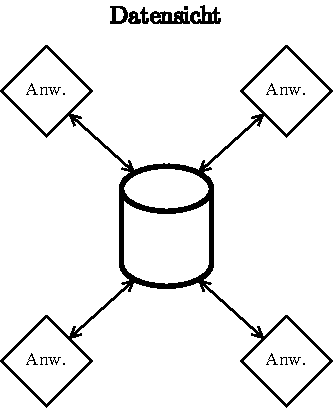
\includegraphics[height=5cm]{./assets/data_view.drawio.pdf}
            \end{subfigure}
        }
        % sammeln zunächst Daten, welche Basis für Anwendungen bilden
        % bspw. benötigt Entw. einer KI zunächst breite Datengrundlage, um zu funktionieren
        % kann nicht erst KI entwickeln und dann Datenspeicher
        % Prozess dreht sich herum
        \caption{Prozess- vs. Daten-Sicht}
    \end{figure}
\end{frame}


\begin{frame}{Einleitung III}
    \begin{itemize}
        \item Daten"=getriebene Prozesse noch nicht in Breite etabliert
        \item kein vollständiges Ausnutzen des Potenzials für Wirtschaft

        \pause
        \item überteuerte, langwierige Projekte, bspw. BER (2,8x Bauzeit, 3x Kosten)~\cite{stalinskiBestBERZahlen2020}
        
        \pause
        \item \enquote{We've \alert{lost control} of our personal data} -- Tim Berners-Lee~\cite{berners-leeThreeChallengesWeb2017}
        
        \pause
        \item[$\Rightarrow$] multilateraler, sicherer, vertrauenswürdiger Datenaustausch + Datensouveränität~\cite{mollerIndustrialDataEcosystems2024}
        \pause
        \begin{itemize}
            \item[$\to$] Data Spaces mit \emph{Solid}~\cite{mecklerWebLinkedData2023}
        \end{itemize}
    \end{itemize}
\end{frame}
